\section{Introduction}
\iftoggle{commentboxes}{% Defined in packages.tex
\gototoc
\begin{tabular}{|p{\linewidth}|}
	\hline
	\begin{itemize}
		\item Improve the literature review part.
		\item Add a reference that explains why EM can default \textit{in LC}: small cost to default in LC if already defaulted in FC, if external debt of firms is large don't want to default in FC.
		\item Review cases of actual default. Papers by Reinhart, database BoC-BoE, S\&P annual report on sovereign defaults.
		\item [Done] Why doing this is useful/necessary? To improve the conduct of MP in EMEs: appropriately characterizing expectations, TP and credit risk.
	\end{itemize}
	\\ \hline
\end{tabular} \\}

What would be the cost for the U.S. to finance in other currencies? For debt issued in the currencies of other advanced economies, the yields paid by the U.S. would likely be similar to the ones paid by their governments. But for debt issued in the currencies of emerging markets, the yields paid by the U.S. would likely be lower than those paid by the respective governments, mainly because of the lower default risk associated with the U.S. This paper exploits this idea to construct risk-free yield curves for emerging markets. I then use them to estimate the term premia embedded in them.

In theory, the yield of a \textit{risk-free} zero-coupon bond can be decomposed into the average short-term interest rates expected over the life of the bond plus a term premium for holding it. The term premium is the compensation investors require for bearing the risk that the short-term interest rate does not evolve as they expect. If long-term bonds are seen as risky, investors require a compensation (i.e. a positive term premium) for holding them. On the contrary, if such bonds are seen as a hedge, investors will be willing to receive less than what is expected for the short-term rate, which translates into a negative term premium.

Estimation of the term premium is an important task in macroeconomics and asset pricing. For instance, term premia estimates provide valuable information for analyzing the transmission of monetary policy. They also allow to study the macroeconomic determinants of bond risk premia and provide an important channel to understand the differences between the sovereign debt markets of advanced and emerging economies. However, the literature has mainly focus on estimating the term premia for advanced economies. Although there are some estimates for emerging markets,\footnote{See, for example, \cite*{DePooter_etal:2013}, and \cite*{BlakeRuleRummel:2015}.} none of them corrects for credit risk.\footnote{Credit risk here is defined broadly including, for example, (selective) default risk, currency convertibility risk, regulation risk, capital controls, jurisdiction risks and liquidity risk. Therefore, when investors require compensation for any of these risks, it is considered that they demand a premium for credit risk even if the country does not default per se. Notwithstanding this, historically emerging markets have indeed defaulted in debt issued in local currency, some examples include El Salvador (2017), Ecuador (2008), Argentina (2001), Russia (1998); in 1999 after an earthquake, Turkey retroactively taxed its debt.} This paper fills that void.

The findings reported below show that the term premia in emerging markets for the 10-year maturity is around 175 basis points on average, and that the U.S. term premium is a common factor influencing them. In addition, domestic inflation and unemployment also play a prominent role in explaining the dynamics of the term premia. An increase in those variables is associated with an increase in the term premia. The exchange rate is also related and its effect is in line with the risk-taking channel of exchange rates found by \citet*{HofmannShimShin:2017}; according to which a currency appreciation is associated with easier financial conditions and compressed sovereign bond spreads.

Affine term structure models are the standard tool to estimate the term premium. A key assumption in those models is that the yields used are free of default risk. Although it is a reasonable assumption for the sovereign debt of advanced countries, that of emerging markets include a premium for credit risk, even for bonds issued in local currency (LC) for which they have (in theory) the ability to print it to repay their debts \citep{DuSchreger:2016a}. Therefore, a direct application of term structure models to sovereign yields of emerging markets would give biased estimates of the term premium. I construct synthetic yield curves using financial derivatives to address this issue. This is important since bonds denominated in LC have become an important source of funds for emerging markets in recent years, in contrast to foreign currency (FC)-denominated bonds \citep{DuSchreger:2016b}. Recent studies have used synthetic instruments in other contexts but, to the best of my knowledge, this is the first attempt to estimate affine term structure models using synthetic yield curves.

To construct the synthetic yield curves, I follow the methodology developed in a series of papers by \cite{DuSchreger:2016a}, \citet*{DuImSchreger:2018} and \citet*{DuImSchreger:2018CIP}. Today an investor can lock in a risk-free investment in LC by first exchanging LC for U.S. dollars (USD), investing those USD in U.S. Treasuries and then entering into a forward contract in which the investor agrees to sell USD for LC in the future. Once the payoff (in USD) from the Treasuries is realized, the investor exchanges USD back into LC at the exchange rate agreed in the forward contract. While the authors use the synthetic LC yield curve as an intermediate step to analyze the deviations from covered interest parity, I focus on the synthetic curve itself and rely on its `risk-free' property to estimate the term premium. This allows me to decompose the LC yield curves into three parts: the expected long-term policy rate, the term premium and the LC credit spread (the difference between the nominal and synthetic curves). The LC credit spread is a measure to assess credit risk in LC debt. Arguably, a better characterization of the three components will enhance the analysis of monetary policy in emerging markets.

This paper is related to different branches of the literature in international macroeconomics and finance. First, it makes use of synthetic LC yield curves which was pioneered by \cite{DuSchreger:2016a} for emerging markets in the context of credit spreads and later used by \citet*{DuImSchreger:2018} for advanced economies to study the convenience yield of U.S. Treasuries. Second, it makes an international comparison of term premia estimates for emerging markets, contributing to the work done by \cite{Wright:2011} for advanced economies.

On the effects of U.S. monetary policy shocks on the yields of emerging markets, this paper is related to the results in \citet*{GilchristYueZakrajsek:2018} by studying not only the effects on the yield curve but on its components. \cite{HofmannShimShin:2017} already study the link between the U.S. monetary policy, the exchange rate and LC credit spreads.

Finally, this paper contributes to the large literature on term structure models by pioneering the use of synthetic yield curves in their analysis.

%Finally, on the relationship between affine term structure models and exchange rates this paper is related to \cite{AngChen:2010}.

The rest of the paper is structured as follows. The next section explains how to construct both nominal and synthetic yield curves. Section \ref{sec:ATSM} explains the affine term structure model that will be estimated. Section \ref{sec:methodology} describes the estimation procedure and the data sources. Section \ref{sec:results} reports and discusses the estimated term premia, while section \ref{sec:correl} studies their cyclical properties. The last section concludes.

\section{Construction LC Yield Curves} 
\iftoggle{commentboxes}{% Defined in packages.tex
\gototoc
\begin{tabular}{|p{\linewidth}|}
	\hline
	\begin{itemize}
		\item Include reference for small counterparty risk in CCS.
	\end{itemize}
	\\ \hline
\end{tabular} \\}

The focus of this paper is on the synthetic yield curve, which will be denoted as $\yLCsynt$; however, the nominal yield curve, $\yLCnom$, is also of interest for comparison purposes and calculate the deviations from covered interest rate parity (CIP). This section explains how to construct both curves.

\subsection{Construction of Synthetic Yield Curves} \label{sec:synYC}
The key idea to construct the synthetic LC yield curves is to swap the U.S. yield curve into LC using the forward premium for the respective maturity \citep*[see][]{DuImSchreger:2018CIP}.

For maturities of less than one year, the forward premium can be calculated as the difference between the forward and the spot exchange rates. Outright forwards, however, become illiquid for longer periods. For maturities greater than one year, the forward premium can be calculated using cross-currency swaps (CCS).\footnote{CCS are used instead of credit default swaps (CDS) for two reasons: the definition of default in CDS is not always straightforward and, more importantly, defaults on LC bonds are not considered trigger events of CDS contracts.}  Although, the fixed-for-fixed CCS rates are rarely observed in the market directly, they can be constructed using cross-currency basis swaps and interest rate swaps. The idea is to swap fixed payments in LC into floating rate USD-cash flows using cross-currency basis swaps (referenced to the USD London interbank offered rate), and then swapping those floating rate cash flows into fixed USD-cash flows using interest rate swaps. CCS are usually collateralized instruments and so the bilateral counterparty risk in CCS is small.

Let $\yUS$ denote the zero-coupon yield for the $\tnr$-period U.S. Treasury bond at time $t$, and $\fwdprm$ the $\tnr$-period forward premium from the USD to the LC at time $t$. Then the zero-coupon synthetic LC yield for the $\tnr$-period bond at time $t$, $\yLCsynt$, is defined as
	\begin{equation} \label{eq:yLCsynt}
	\eqyLCsynt .
\end{equation}

Note that $\yLCsynt$ is the borrowing rate paid by a hypothetical risk-free issuer in LC, it is the $\tnr$-period synthetic LC risk-free funding rate. It is worth mentioning that the resulting synthetic yield curve $\yLCsynt$ does not require knowledge of the nominal yield curve, $\yLCnom$.\footnote{Using equivalent notation for the U.S., we then have that $\yUSsynt = \yUS$.}

According to the CIP condition, the synthetic and direct LC interest rates should be equalized. In particular, a sovereign issuer of an emerging market should be able to borrow directly or indirectly (synthetically) in LC at the same yield. However, \cite*{DuTepperVerdelhan:2018} show that there are persistent and systematic deviations from CIP. In fact, \cite{DuSchreger:2016a} and \cite{DuImSchreger:2018} study these deviations for emerging markets and advanced economies, respectively. In particular, the spread between the two yields ($\yLCnom - \yLCsynt$) is what \cite{DuSchreger:2016a} define as the LC credit spread for emerging markets, and what \cite{DuImSchreger:2018} called the convenience yield for advanced countries.

\subsection{Construction of Nominal Yield Curves}
I use Bloomberg Fair Value (BFV) curves to estimate the nominal yield curve, $\yLCnom$. BFV curves are par yield curves provided by Bloomberg on a daily basis for different maturities. To obtain the implied zero-coupon curves, the yields are converted into discount factors, which are then used to estimate the parameters of the Nelson-Siegel-Svensson model.\footnote{As a robustness check, I estimate the nominal yield curves from actual prices for some countries, they follow those reported by Bloomberg closely.}

%\subsection{Estimation of Synthetic Yield Curves} \label{sec:synthEstim}
%The methods to estimate the yield curve at a particular point in time can be classified in parametric and non-parametric. Since the purpose of estimating the yield curve in this paper is to understand its determinants, a parametric approach is more convenient because it smooths through idiosyncratic variation and, notwithstanding, it allows for a variety of yield curve shapes. This approach is also followed for the U.S. by \citet*{GSW:2007}. 

\cite{NelsonSiegel:1987} assume that the instantaneous forward rate $\tnr$ years ahead follows a continuous function that depends on four parameters:
	\begin{equation} \label{eq:NSfwd}
	\fInst = \betaLT + \betaST \loadSTnsFwd + \betaMTns \loadMTnsFwd.
\end{equation}

The behavior at long and short maturities is determined by the parameters $\betaLT$ and $\betaST$, while $\betaMTns$ and $\tauNS$ determine the magnitude, direction and position of the yield curve's ``hump".

\cite{Svensson:1994} extends the Nelson-Siegel approach to allow for a second hump at longer maturities. This is achieved at the expense of introducing two more parameters in the functional form of the instantaneous forward rate as follows:
	\begin{equation} \label{eq:NSSfwd}
	\fInst = \betaLT + \betaST \loadSTnsFwd + \betaMTns \loadMTnsFwd
	+ \betaMTnss \loadMTnssFwd.
\end{equation}

The continuously compounded zero-coupon yield curve implied by the Svensson model is obtained by integrating the instantaneous forward rate in equation \ref{eq:NSSfwd}:\footnote{Note that the Nelson-Siegel model is obtained by setting $\betaMTnss$ equal to zero.}
	\begin{equation} \label{eq:NSSzero}
	\begin{split}
		\yZero = \betaLT + \betaST \left(\loadSTnsZero\right) 
		& + \betaMTns \loadMTnsZero \\
		& + \betaMTnss \loadMTnssZero.
	\end{split}
\end{equation}

The parameters in the Svensson model are estimated by minimizing the sum of squared deviations between the prices obtained from the observed $\yLCnom$ and the prices implied by equation (\ref{eq:NSSzero}) weighted by the inverse of the duration for each period. Using price deviations weighted by duration is approximately equal to fitting yields but is faster because the latter requires to numerically find the root to a nonlinear equation.

\section{Affine Term Structure Model} \label{sec:ATSM}
\iftoggle{commentboxes}{% Defined in packages.tex
\gototoc
\begin{tabular}{|p{\linewidth}|}
	\hline
	\begin{itemize}
		\item A
	\end{itemize}
	\\ \hline
\end{tabular} \\}

Discrete-time affine term structure models with an exponentially affine pricing kernel are commonly used in the literature to estimate the dynamics of the yield curve and the term premium, mainly for advanced economies \citep[see][]{Wright:2011}. In this paper, however, I use an affine term structure model to estimate the dynamics of the synthetic yield curve. The advantage of doing it is to decompose the \textit{nominal} yield curve into three parts: the expected future short-term interest rate, a term premium and the LC credit spread.

\subsection{Model} \label{sec:ATSM_eqns}
Let $\Pzero$ be the price at time $t$ of a zero-coupon bond with maturity $\tnr$, then the continuously compounded yield on that bond is $\yZero = - \ln \Pzero/\tnr $. The one-period continuously compounded risk-free rate is thus $\rShort = - \ln P_{1,t}$.

The no-arbitrage assumption implies that there exists a stochastic discount factor (SDF) $\SDF$ such that today's price equals the expectation of tomorrow's discounted price:
	\begin{equation} \label{eq:Pzero}
	\Pzero = \Expec \left[ \SDF \Pzerolag \right].
\end{equation}
Since the price at maturity of a zero-coupon bond is $1$, recursive substitution of equation (\ref{eq:Pzero}) implies that today's price equals the expectation of the product of SDFs over the life of the bond, $\Pzero = \SDFprod$.

A $\Xdim \times 1$ vector of state variables $\Xvars$ is assumed to drive the dynamics of the one-period interest rate $\rShort$, the $\Xdim \times 1$ market price of risk $\riskprice$ and the logarithm of the SDF $\SDF$ in an affine way as follows:
	\begin{equation} \label{eq:rShort}
	\rShort = \deltazero + \deltaone' \Xvars
\end{equation}
	\begin{equation} \label{eq:riskprice}
	\riskprice = \lambdazero + \lambdaone \Xvars
\end{equation}
	\begin{equation} \label{eq:SDF}
	\SDF = \exp\left( -\rShort -\frac{1}{2} \riskprice'\riskprice - \riskprice'\error \right)
\end{equation}

where $\error$ is $i.i.d.$ $\Normal \left(0,I_{\Xdim}\right)$. Note that the SDF is conditionally lognormal and heteroskedastic.

Assume that the dynamics of the vector of state variables $\Xvars$ evolve under the physical measure $(\Pmeasure)$ according to the following vector autoregression (VAR):
	\begin{equation} \label{eq:XvarsP}
	\XvarsFwd = \Xmu + \XPhi \Xvars  + \XSigma \error .
\end{equation}

The SDF in equation (\ref{eq:SDF}) and the law of motion of the vector of state variables in equation (\ref{eq:XvarsP}) can be formalized separately or jointly, see \cite{GurkaynakWright:2012} for a review of the literature.

The following parameters:
	\begin{equation*} 
	\XmuStar = \Xmu - \XSigma \lambdazero
\end{equation*}
	\input{../Equations/XPhiStar}

govern the dynamics of the vector of state variables under the risk-neutral or pricing measure $(\Qmeasure)$:
	\begin{equation} \label{eq:XvarsQ}
	\XvarsFwd = \XmuStar + \XPhiStar \Xvars  + \XSigma \error.
\end{equation}

The log price and the continuously compounded yield of a risk-free zero-coupon bond in this model are then affine functions of the state variables $\Xvars$:
	\begin{equation*}
	\Pzero = \exp\left( \affineA + \affineB \Xvars \right)
\end{equation*}
	\begin{equation} \label{eq:yAffine}
	\yZero = - \frac{\affineA}{\tnr} - \frac{\affineB}{\tnr} \Xvars .
\end{equation}
where the scalar $\affineA = A(\deltazero, \deltaone, \XmuStar, \XPhiStar, \XSigma)$ and the $1 \times \Xdim$ vector \input{../Equations/functionBn}.

The coefficients can be computed recursively combining the no-arbitrage condition and the functional form for bond prices as follows
	\begin{equation*}
	\affineAfwd = \affineA + \affineB' \XmuStar + \frac{1}{2} \affineB' \XSigma \XSigma' \affineB - \deltazero , \quad A_{0} = 0
\end{equation*}
	\begin{equation*}
	\affineBfwd = - \deltaone + \XPhiStar{'} \affineB , \quad B_{0} = 0
\end{equation*}

The term premium can then be estimated as the difference between the yields obtained under the $\Qmeasure$ measure and the yields obtained under the $\Pmeasure$ measure.
	\begin{equation} \label{eq:TPatsm}
	\TPatsm = \yZero^\Qmeasure - \yZero^\Pmeasure.
\end{equation}

Note that a key assumption behind this model is that $\yZero$ is risk-free rate. \cite{DuSchreger:2016a} show that $\yLCnom$ for emerging markets is not risk-free since the LC credit spread is statistically different from zero. Therefore, focusing on $\yLCsynt$ better aligns with the risk-free assumption.

\subsection{Identification Problem} \label{sec:Identification}
In principle, the only input needed to estimate the parameters of the affine term structure model are zero-coupon bond yields. This is enough to estimate ($\XmuStar, \XPhiStar$), the pricing coefficients under $\Qmeasure$ in equation (\ref{eq:XvarsQ}). However, they are not enough to identify ($\Xmu, \XPhi$) the parameters under $\Pmeasure$ in equation (\ref{eq:XvarsP}), which are necessary to estimate the term premium as indicated by equation (\ref{eq:TPatsm}).

This identification problem is due to the high persistence of bond yields, which results in small sample bias as has been highlighted by \cite{KimOrphanides:2012} and \cite{Guimaraes:2014}. The dynamics of the state vector will then tend to mean-revert too quickly, overestimating the stability of the expected path of the short-term interest rate. In that situation much of the variability in yields will be attributed to fluctuations in the term premium. The problem intensifies with the persistence in the data. Since daily data is highly persistence, affine term structure models are usually estimated using monthly data.

Different solutions have been proposed to address the identification problem, including restrictions on parameters, bias-corrected estimators and using of survey forecasts of professional forecasters. \cite{Guimaraes:2014} compares the three approaches and concludes that the use of surveys is an effective solution to obtain robust decompositions of the yield curve.\footnote{In a future draft, I will therefore supplement the affine term structure model with survey data on the expected long-term policy rate for each country.}

Therefore, there are two ways in which the information from surveys can be used in this context. First, to obtain a model-free estimate of the term premium as the difference between the long-term interest rate and the expected future short-term interest rate over the same horizon obtained from surveys, which serves as a robustness check. Second, to supplement the information from bond yields in the estimation of affine term structure models.

\section{Methodology} \label{sec:methodology}
This section describes both the estimation method and the data sources employed in the estimation of the model presented in section \ref{sec:ATSM_eqns}.

\subsection{Estimation} \label{sec:Estimation}
Affine term structure models can be estimated by maximum likelihood. Traditionally, the convergence to the global optimum of that method has been subject to computational challenges and multiple local optima. \citet*{JSZ:2011} (hence JSZ), however, propose a normalization that improves the convergence to the global optimum of the likelihood function.

The model's likelihood function is the product of the $\Pmeasure$ and $\Qmeasure$ likelihood functions. The JSZ normalization allows for the near separation of both likelihood functions and reduces the dimension of the parameter space from $(\deltazero, \deltaone, \XmuStar, \XPhiStar, \XSigma)$ to $(r^{\Qmeasure}_{\infty}, \lambda^{\Qmeasure},\XSigma)$, where $r^{\Qmeasure}_{\infty}$ is the long-run short-term interest rate under $\Qmeasure$, $\lambda^{\Qmeasure}$ is a $\Xdim \times 1$ vector of ordered eigenvalues of $\XPhiStar$, and $\XSigma$ is a lower triangular matrix with positive diagonal elements.

The JSZ normalization allows a two-stage estimation of the model presented in section \ref{sec:ATSM_eqns}. First, the $\Pmeasure$ parameters are estimated by running OLS on the VAR in equation (\ref{eq:XvarsP}) using the estimated $\Xdim$ principal components of the synthetic yield curve $\yLCsynt$. This provides initial values for the maximum likelihood estimation of the matrix $\XSigma$. Then, taking $\hat{\Xmu}$ and $\hat{\XPhi}$ as given, the $\Qmeasure$ parameters can be estimated by maximum likelihood.


%The model described above can be estimated in a few simple steps. First, equation (\ref{eq:XvarsP}) is estimated by OLS to obtain estimates of $\Xmu$, $\XPhi$ and $\XSigma$. The estimates of $\deltazero$ and $\deltaone$ can be obtained by estimating equation (\ref{eq:rShort}) also by OLS. Finally, the estimates of $\lambdazero$ and $\lambdaone$ are obtained by minimizing the distance between the fitted yields from equation (\ref{eq:NSSzero}) and the yields implied by the affine model in equation (\ref{eq:yAffine}). More robust methods to estimate the model are available,\footnote{For example, \citet*{JSZ:2011} and \cite{HamiltonWu:2012} use maximum likelihood, \cite{Duffee:2011b} uses the Kalman filter, while \citet*{ACM:2013} use linear regressions.\label{fn:est_methods}} and one of them will be used in future versions of this paper.
%
%However, in order to obtain preliminary estimates of the term premium only equations (\ref{eq:rShort}) and (\ref{eq:XvarsP}) are used in this version. To obtain estimates of the expected short-term interest rates in future periods, the expectation of the vector of state variables $\Xvars$ (which can be computed by iterating forward equation (\ref{eq:XvarsP})) is substituted in equation (\ref{eq:rShort}). The expectation of a yield $\tnr$ periods ahead is then obtained as the average of the expected short-term rates over $\tnr$ periods. The term premium estimate is then computed as the difference between the nominal yield and the expected yield obtained in this way.

\subsection{Data}
The macroeconomic and financial variables used in section \ref{sec:correl} are downloaded from Bloomberg. Below I describe the data sources for the construction of the yield curves and for the surveys of professional forecasters.

\subsubsection{Yield Curve Data}
I use end-of-month data for the following 15 emerging markets (EMs):\footnote{The currency identifier for each country is shown in parenthesis.} Brazil (BRL), Colombia (COP), Hungary (HUF), Indonesia (IDR), Israel (ILS), Korea (KRW), Malaysia (MYR), Mexico (MXN), Peru (PEN), Philippines (PHP), Poland (PLN), Russia (RUB), South Africa (ZAR), Thailand (THB) and Turkey (TRY). 

In order to establish a set of stylized facts for emerging markets, the results are compared against those obtained for 10 advanced countries (AEs): Australia (AUD), Canada (CAD), Denmark (DKK), Germany (EUR), Japan (JPY), Norway (NOK), New Zealand (NZD), Sweden (SEK), Switzerland (CHF) and the United Kingdom (GBP). For some comparisons, these countries are split into two groups to assess whether the type of advanced country matters. The first group (G-3) is comprised by Germany, Japan and the United Kingdom. The second group (A-SOE) comprises the rest of the countries. Note that the latter is basically a group of advanced small open economies, which can be more directly comparable to emerging markets.

As explained in section \ref{sec:synYC}, the U.S. yield curve and the forward premium for different maturities are needed to construct the LC synthetic yield curves. Data for the U.S. zero-coupon yield curve is obtained from the database developed by \citet*{GSW:2007} (hence GSW). Although the GSW dataset goes back to 1961, the main issue for the analysis is the information needed to calculate the forward premium. 

As mentioned before, for periods less than one year the forward premium is calculated using forward exchange rates, while for longer periods it is calculated from CCS rates. The maturities of less than one year considered in the analysis are 3, 6 and 9 months; that is, I use the forwards and the spot exchange rate to compute the forward premium for those maturities. To construct the CCS rates, I use each available year starting from year one. The maximum maturity available varies per country but there is data covering at least up to ten years; for some countries, it can go as far as 30 years.\footnote{After 10 years, the periodicity decreases to every five years. Then, when they are available, the maturities beyond 10 years are usually for 15, 20, 25 and up to 30 years.} %This is taken into account when estimating the model in section \ref{sec:synthEstim}. Yield curves with maturities up to 10 years tend to exhibit one hump at most. The Nelson-Siegel model can capture that pattern in a more parsimonious way than the Svensson model. Therefore, the Svensson model is only estimated when there are at least three maturities beyond 10 years.

The forwards used to construct the forward premiums for less than one year for Korea, Philippines and Thailand is obtained from Datastream. For all the other countries, the data to construct the forward premiums (using forwards and CCS curves) is obtained from Bloomberg. A spreadsheet with the Datastream and Bloomberg tickers used in the construction of the forward premiums as well as the nominal yield curves is available upon request.\footnote{The file consolidates and expands (with tenors and tickers) equivalent files kindly posted online in Wenxin Du and Jesse Schreger's websites.}

The model in section \ref{sec:ATSM_eqns} is estimated for each country separately. Therefore, the starting dates vary (between January 2000 and November 2006) but the end date is the same for all countries (January 2019). Although data for advanced countries is available earlier, their initial dates are set at January 2000. Note that there are at least 10 years of data for all emerging markets, which is a reasonable time period for the estimation of affine term structure models.
%Table \ref{tab:start_dates} shows the earliest end-of-month dates with available data for emerging countries.
%	\begin{table}
	\centering
%\begin{tiny}
	\begin{tabular}{lc}
\toprule
\textbf{Country}&\textbf{End-of-Month}\\\midrule
{ COP}&30-Jun-2005\\\
HUF&31-Oct-2006\\\
IDR&30-Mar-2001\\\
ILS&28-Feb-2006\\\
MXN&28-Nov-2003\\\
PEN&31-Jul-2006\\\
PHP&31-Jan-2000\\\
PLN&31-Mar-2005\\\
TRY&31-May-2005\\\
KRW&31-Jan-2000\\\
MYR&29-Dec-2006\\\
RUB&28-Apr-2006\\\
THB&30-Nov-2006\\\
ZAR&29-Feb-2000\\ \bottomrule
\end{tabular}
\\
\caption{Starting Dates per Country.}\label{tab:start_dates}
%\end{tiny}
\end{table}

\subsubsection{Survey Data} \label{sec:SurveyData}
As mentioned in section \ref{sec:Identification}, long-horizon forecasts for the policy rate of emerging markets can be used to obtain model-free estimates of the term premium and to supplement the information from bond yields to estimate the affine term structure models.

Although Consensus Economics provides long-horizon forecasts for consumer inflation and real GDP growth, it does not provide those forecasts for policy rates. In order to approximate the policy rate expectations embedded in those survey responses, I use the following model for the policy rate of each emerging market
	\begin{equation} \label{eq:TaylorRule}
	\rShort = \beta_{0} + \beta_{\STrate} \rShortlag + \beta_{\pi} \pi_{t} + \beta_{y} g_{t} + \epsilon_{t},
\end{equation}

where $\rShort$ is the policy rate, $\pi_{t}$ is the year-on-year consumer inflation and $y_{t}$ is the year-on-year real GDP growth. $\beta_{\STrate}$ is a smoothing parameter that improves the fit of the model to the data. The information for $\rShort$ is obtained from the policy rate statistics of the Bank for International Settlements, while the data for consumer inflation and real GDP growth is downloaded from Bloomberg.

To obtain the implied expectations of the policy rate, I estimate the regression in equation (\ref{eq:TaylorRule}) using quarterly data and assume that the parameter estimates apply to the long-horizon survey forecasts for inflation and real GDP growth from Consensus Economics. I do this for all emerging markets in the sample except for Israel and South Africa due to data availability.

The expectations of the policy rate obtained in this way can then be used for the two goals described above. In particular, the term premium using surveys will be obtained as\footnote{Note that under stationarity, $\mathrm{E}(\rShort) = \mathrm{E}(\rShortlag)$.}
	\input{../Equations/TPsurvey}


\section{Empirical Results} \label{sec:results}
\iftoggle{commentboxes}{% Defined in packages.tex
\gototoc
\begin{tabular}{|p{\linewidth}|}
	\hline
	\begin{itemize}
		\item Add website for Excel file with tickers.
		\item Units or deviation with respect to what for RMSE table.
		\item Include summary statistics of the ATSM fitted curves to give a feeling about the data.
		\item Include macro factors when estimating the dynamics of the vector of state variables in equation \ref{eq:XvarsP}.
		\item When considering the spillover effects of the monetary policy in the U.S., use a better measure of shocks (e.g. changes in futures of the fed funds rate around monetary policy announcements) and differentiate conventional from unconventional monetary policy.
	\end{itemize}
	\\ \hline
\end{tabular} \\}

The aim of this paper is to decompose the synthetic yield curves of emerging markets, which in turn will provide a decomposition of their nominal yield curves. I use two benchmarks to assess the relevance of the results. First, since emerging markets are mainly small open economies, I compare their estimated term premia to those of advanced small open economies. Second, I compare the term premia obtained from both nominal and synthetic yield curves; in each case, assuming the the curve used is risk-free.

\subsection{Estimated Synthetic Yield Curves}
An affine term structure model is estimated for each country using the JSZ normalization and the two-stage procedure described in section \ref{sec:Estimation}. The VAR model in equation (\ref{eq:XvarsP}) is estimated using the first three principal components (PCs) of the synthetic yield curve. Consistent with the empirical evidence that uses nominal yield curves,\footnote{\cite{LittermanScheinkman:1991} first report this and refer to those PCs as level, slope and curvature.} on average more than $99\%$ of the variation in synthetic yields is explained by those three factors for all emerging markets.
%	\begin{table}
	\centering
	\begin{tabular}{lcccc}
		\toprule
		\textbf{Country}&\textbf{PC1}&\textbf{PC2}&\textbf{PC3}&\textbf{Sum}\\\midrule
		{ COP}&91.99& 7.14& 0.77&99.91\\\
		HUF&97.33& 2.27&  0.33&99.94\\\
		IDR&92.27&  6.41& 1.20&99.88\\\
		ILS&93.35&  5.23& 1.29&99.88\\\
		MXN&96.25& 3.28& 0.41&99.95\\\
		PEN&79.37&18.70& 1.63&99.7\\\
		PHP&93.97&5.64&0.33&99.95\\\
		PLN&92.22& 6.52& 1.08&99.83\\\
		TRY&96.99& 2.76& 0.19&99.96\\\
		KRW&94.53& 4.71& 0.63&99.88\\\
		MYR&84.005&13.74& 1.85&99.6\\\
		RUB&94.14& 5.33&0.46&99.94\\\
		THB&82.83& 15.52& 1.20&99.56\\\
		ZAR&90.82& 7.865&  1.14&99.83\\ \bottomrule
	\end{tabular}
	\\
	\caption{Proportion of Total Variance in Yields Explained by First 3 PCs.}
	\label{tab:pc_explained}
\end{table}


Table \ref{tab:rmse_atsm} summarizes the fit of the models. The table shows the average root mean square fitting error in annualized percentage points of nominal and synthetic yields for emerging markets and advanced economies.\footnote{For each country, the root mean square fitting error is calculated as the square root of the average (across months and maturities) squared difference between the observed yields and the fitted yields from the estimated affine term structure model.} As can be seen, the fit of the model for the nominal curves of both groups of countries is similar. The fit for the synthetic curves of advanced countries slightly improves relative to the fit for their nominal curves, while that for emerging markets declines. It is worth mentioning that the latter is driven mainly by two countries, Brazil and Indonesia, whose root mean square fitting error is slightly above 2\%.\footnote{Although not as high, the root mean square fitting error for Peru and Philippines is also above average at around 0.64 and 0.54, respectively.} This requires further inspection of the synthetic yield curves of these two countries.\footnote{In some special cases, outliers may need to be dropped in some periods to be able to fit the curve for the rest of the points.} 
	\begin{tiny}\begin{table}\centering\begin{tabular}{l|cc}\toprule & Nominal & Synthetic \\\midrule EM & 0.15 & 0.48 \\AE & 0.13 & 0.08 \\\bottomrule\end{tabular}\caption{Fit of Affine Term Structure Models.}\label{tab:rmse_atsm}\end{table}\end{tiny}
%	\begin{table}
	\centering
	\begin{tabular}{lc}
\toprule
\textbf{Country}&\textbf{RMSE}\\\midrule
{ COP}&0.081\\\
HUF&0.066\\\
IDR&0.112\\\
ILS&0.056\\\
MXN&0.03\\\
PEN&0.167\\\
PHP&0.101\\\
PLN&0.031\\\
TRY&0.056\\\
KRW&0.043\\\
MYR&0.052\\\
RUB&0.078\\\
THB&0.031\\\
ZAR&0.041\\ \bottomrule
	\end{tabular}
	\\
	\caption{Average RMSE of Nelson-Siegel Fit.}\label{tab:rmse_ns}
\end{table}

%The implied yields obtained in this way are then used to estimate the term structure model as explained in section \ref{sec:Estimation}. For example, when data is not available to compute equation (\ref{eq:yLCsynt}) for $\tnr = 0.25$, equation (\ref{eq:rShort}) is estimated using the Nelson-Siegel implied 3-month yields.

\subsection{Nominal Yield Curve Decomposition}
Once the affine term structure model is estimated for each country, I can compute the term premia for each maturity as explained in section \ref{sec:ATSM_eqns}.\footnote{Although term premia estimates are calculated for all maturities, only the $10$-year maturity is reported in what follows for the sake of brevity.} This allows to decompose both the synthetic as well as the nominal yield curves. Table \ref{tab:decomp10yr} shows the average across countries of the decomposition of the $10$-year yields.\footnote{The numbers in the table do not add up exactly for two reasons: (1) the term premium is obtained using equation (\ref{eq:TPatsm}), that is it uses the fitted synthetic yield curve, while the table reports the observed synthetic yield curve for the column `Synthetic', and (2) the sample period for the yield curves might differ slightly to that of the LC credit spread.} Several patterns emerge from the table. The values for the deviations from CIP (CIP Dev) are in line with the results reported by \cite{DuSchreger:2016a} and \cite{DuImSchreger:2018} referred to as the LC credit spread (LCCS) for emerging markets and the convenience yield for advanced countries, respectively. Note, however, that the estimated term premium is higher on average than the CIP dev for the three groups of countries; it is almost 90 basis points higher for emerging markets, almost 150 basis points higher for Germany, Japan and the United Kingdom and more than 200 basis points for the advanced small open economies. To assess whether the term premium and the CIP Dev are statistically different from each other, I perform a $t$-test for the equality of means (with unequal variances) between them. The null of equal means is rejected at the $5$\% significance level for all countries except Korea, Russia and Turkey.
	\begin{tiny}\begin{table}\centering\begin{tabular}{l|ccccc}\toprule & Nominal & Synthetic & Expected & Term Premium & CIP Dev \\\midrule EM & 7.10 & 6.11 & 4.29 & 1.74 & 0.85 \\A-SOE & 3.48 & 3.52 & 1.54 & 1.97 & -0.23 \\G-3 & 2.41 & 2.13 & 0.52 & 1.60 & 0.15 \\\bottomrule\end{tabular}\caption{10-Year Yield Decomposition (\%).}\label{tab:decomp10yr}\end{table}\end{tiny}
%	\begin{tiny}\begin{table}\centering\begin{tabular}{l|cccccc}\toprule & N & Actual & Synthetic & Expected & TP & LCCS \\\midrule BRL & 141 & - & 8.55 & 7.00 & 1.55 & - \\COP & 154 & 8.82 & 7.09 & 4.90 & 2.19 & 1.06 \\HUF & 138 & 6.60 & 4.45 & 3.33 & 1.12 & 1.54 \\IDR & 205 & 9.36 & 9.31 & 8.39 & 0.92 & 0.73 \\ILS & 146 & 4.61 & 3.45 & 1.46 & 2.00 & 0.75 \\MXN & 173 & 7.51 & 7.00 & 5.36 & 1.64 & 0.33 \\PEN & 141 & 6.00 & 5.47 & 2.94 & 2.53 & 0.46 \\PHP & 219 & 7.94 & 7.41 & 5.57 & 1.84 & 0.76 \\PLN & 157 & 5.75 & 3.89 & 2.66 & 1.23 & 0.79 \\TRY & 155 & 10.97 & 10.34 & 10.87 & -0.53 & 0.57 \\KRW & 219 & 4.60 & 3.54 & 2.48 & 1.06 & 1.03 \\MYR & 136 & 4.24 & 3.21 & 2.33 & 0.88 & 0.77 \\RUB & 144 & 8.38 & 8.24 & 8.11 & 0.13 & 0.07 \\THB & 137 & 4.08 & 2.94 & 1.73 & 1.20 & 0.63 \\ZAR & 218 & 9.10 & 8.83 & 7.80 & 1.03 & 0.21 \\\bottomrule\end{tabular}\caption{LC Decomposition, 10-Year: Average Values.}\label{table:Decomp10yr}\end{table}\end{tiny}

For emerging markets, the main component of the nominal yield curve is the expectation of the future short-term interest rate; for advanced countries, the main component is the term premium. Note also that for the subset of small open economies it is cheaper to borrow directly in their own currency (since CIP Dev is negative), unlike what is seen for emerging markets.

\subsection{Term Premia: Nominal or Synthetic Yield Curve?}
Affine term structure models are usually estimated using nominal yield curves on the assumption that they are free of default risk. \cite{DuTepperVerdelhan:2018} show that deviations from covered interest parity are non-negligible. Therefore, there is a wedge between the nominal ($\yLCnom$) and synthetic ($\yLCsynt$) yield curves given by the LCCS in the case of emerging markets and by the convenience yield in the case of advanced economies. Does this wedge alters the estimated term premia? Equivalently, does it matter which curve is used to estimate the term premia? We can answer these questions by fitting the model described in section \ref{sec:ATSM_eqns} to both curves.

Table \ref{tab:tp_compare10yr} show the average term premia across groups of countries obtained by using the nominal and the synthetic yield curves. For advanced countries the difference between the two is less than 10 basis points, while that for emerging markets is more than 40 basis points. Similar to the comparison between the term premia and the CIP Dev, I run a $t$-test of equality of means (with unequal variance) for each country to assess whether the term premia from the two curves are statistically different from each other. The null of equal means is rejected at the $5$\% significance level for all emerging markets except Hungary and Malaysia. However, the null is only rejected for four advanced economies (Australia, Denmark, Japan and New Zealand). This shows that there are gains by using synthetic yield curves to account for credit risk when estimating the term premia, especially for emerging markets.
	\begin{tiny}\begin{table}\centering\begin{tabular}{l|cc}\toprule & Nominal & Synthetic \\\midrule EM & 2.17 & 1.74 \\A-SOE & 2.03 & 1.97 \\G-3 & 1.70 & 1.60 \\\bottomrule\end{tabular}\caption{10-Year Term Premium Comparison (\%).}\label{tab:tp_compare10yr}\end{table}\end{tiny}

The evidence in tables \ref{tab:decomp10yr} and \ref{tab:tp_compare10yr} shows that, although sometimes used interchangeably, the terms `risk premium' and `term premium' are not the same thing, at least not for emerging markets, since \textit{both} the term premium and the LC credit spread play an important role in the dynamics of the risk premium in the bond markets of emerging economies.

\subsection{Stylized Facts of EM Term Premia}
I use the U.S. term premium as a benchmark to compare the behavior of the term premia in emerging markets. Two frequently cited estimates of the U.S. term premium are \cite{KimWright:2005} (hence KW) and \cite*{ACM:2013}. Analysis of those estimates shows that: (1) the U.S. term premium is time-varying; (2) it has declined over time; and (3) it has changed sign in recent years. Common explanations for the decline in the U.S. term premium include an increased demand of U.S. assets by global investors and the effects of the unconventional monetary policy of the Federal Reserve. \cite*{CampbellSunderamViceira:2017} argue that the change in the sign of the term premium from positive to negative is explained by the flip in the sign of the correlation between stocks and bonds; when investors changed their perception of bonds as hedges of investments in stocks, the correlation between the two assets turns negative which drives down the term premium. Finally, the U.S. term premium increases during periods of uncertainty and vice versa; for instance, it increased around the onset of the Great Recession (September 2008), the taper tantrum (June 2013), and the 2016 U.S. presidential election (November 2016), while it declined after the first unexpected announcement of the quantitative easing program by the Fed (March 2009).

The 10-year term premia estimates for emerging markets are plotted in Figure \ref{fig:temp_tp10yrEM}. It is worth highlighting some regularities observed in the figure: (1) term premia in emerging markets are time-varying; (2) the estimates are sensible, i.e. they are mostly positive in most cases fluctuating between $-1$\% and $6$\%; (3) there appears to be co-movement in the term premia of some countries; (4) they behave similar to the U.S. term premium around key dates; (5) there is a slight downward trend in the term premia of some countries; (6) the term premia in emerging markets can be negative during some periods.
%\footnote{In fact, inverted yield curves, which may explain this, are common for some of the countries considered.}
		\begin{figure}[!htbp]
		\begin{centering}
			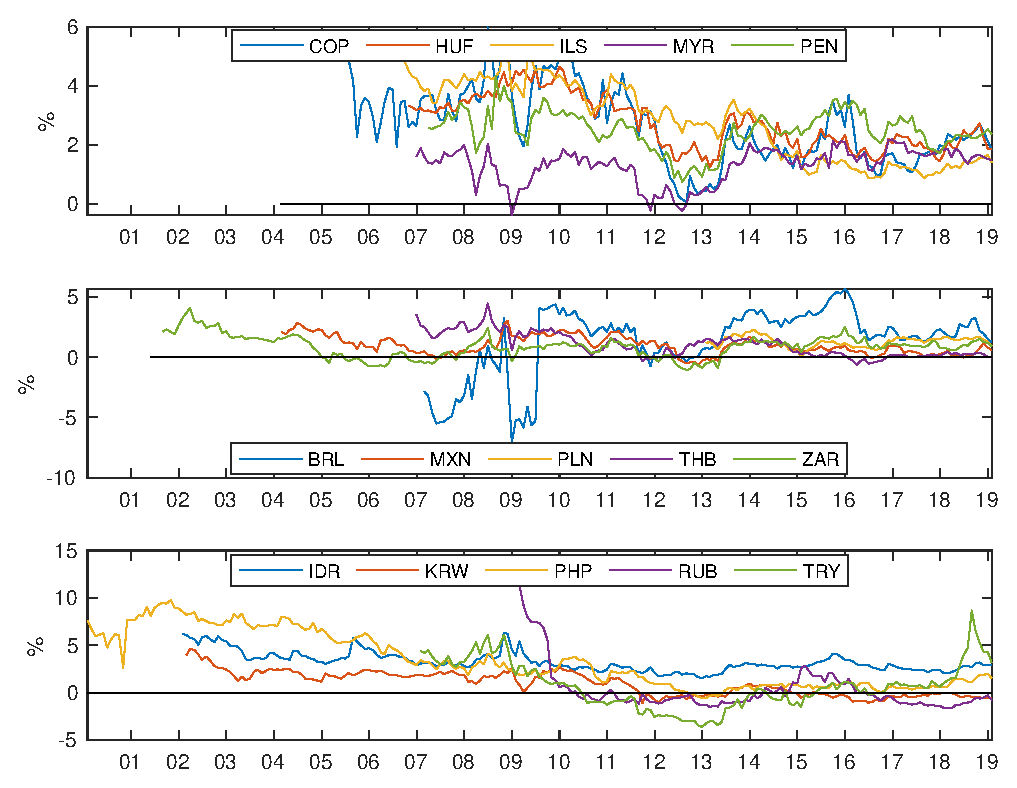
\includegraphics[width=1\textwidth,height=0.7\textheight]{../Figures/Temp/temp_tp10yrEM}
			\par\end{centering}
		\caption{Estimated 10-Year Term Premia: Emerging Markets.}\label{fig:temp_tp10yrEM}
	\end{figure}

Special cases include that of Brazil around the Great Recession and Russia whose term premium declined considerably to turn even negative. These cases seem to reflect local conditions. As is the case for Turkey more recently, where relevant events in 2018\footnote{On June 24, 2018, Recep Tayyip Erdogan won the presidential election. On October 2, 2018, the journalist Jamal Khashoggi disappeared after he visited the consulate of Saudi Arabia in Istanbul.} translated into an increase in its term premium.

 In addition to Brazil, Russia and Turkey, the term premia of most Asian countries has been in negative territory for some period of time. Moreover, with the exception of Brazil and South Africa, negative term premia in emerging markets is a phenomenon observed after the Great Recession.

%To summarize the figure, Table \ref{tab:rp_stats} shows the mean of the 5-year synthetic yields and summary statistics for the estimated 5-year term premia. The means of the synthetic yields fluctuate between $2.3\%$ and $10.5\%$, while the means of the risk premia fluctuate between $-36$ basis points to $150$ basis points. On average, the term premium represents around $12\%$ of the synthetic 5-year yield. For Indonesia, Russia, South Africa and Turkey the standard deviation of their term premia is relatively high compared to their mean. Philippines and Russia had periods with a really negative term premia in October 2000 and the first half of 2015, respectively; excluding those episodes, the term premium has fluctuated between $-3.5\%$ and $5.5\%$.
%	\begin{table}
	\centering
\begin{tabular}{l|cccccc}
\toprule
\multicolumn{1}{c}{}& &\textbf{Yield}&\multicolumn{4}{c}{\textbf{Risk Premium}}\\
\cmidrule(l{.9em}r{.9em}){4-7}
%\cmidrule(lr){3}  \cmidrule(lr){4-7}
\multicolumn{1}{c}{}&\textbf{Obs}&\textbf{Mean}&\textbf{Mean}&\textbf{Std}&\textbf{Min}&\textbf{Max}\\\midrule
{ COP}&154&6.23&1.33&1.21&-0.96&4.41\\\
{HUF}&138&3.71&0.31&0.67&-0.95&1.50\\\
{IDR}&205&8.97&0.52&1.03&-3.06&3.92\\\
{ILS}&146&2.35&1.01&0.63&0.23&2.78\\\
{MXN}&173&6.22&0.88&0.74&-0.62&2.41\\\
{PEN}&141&4.64&1.50&1.55&-3.46&5.54\\\
{PHP}&219&6.54&1.21&1.25&-11.34&3.69\\\
{PLN}&157&3.33&0.64&0.52&-0.61&1.80\\\
{TRY}&155&10.52&-0.36&1.34&-3.22&2.29\\\
{KRW}&219&3.00&0.54&0.72&-1.09&3.51\\\
{MYR}&136&2.67&0.36&0.43&-0.66&1.31\\\
{RUB}&144&7.87&-0.13&1.88&-8.87&3.90\\\
{THB}&137&2.40&0.64&0.79&-1.03&2.89\\\
{ZAR}&218&8.38&0.45&1.12&-3.02&2.25\\ \bottomrule
\end{tabular}
\\
\caption{Summary Statistics: 5-Year Yield and Risk Premium.}\label{tab:rp_stats}
\end{table}

For comparison purposes, Figure \ref{fig:temp_tp10yrAE} shows the 10-year term premia estimates for advanced economies using synthetic yield curves. A clear downward trend is observed for all countries. This is consistent with the empirical evidence that uses nominal yield curves; \cite{Wright:2011} shows  a declining trend in term premia for most of these countries going back to the 1990s.
		\begin{figure}[!htbp]
		\begin{centering}
			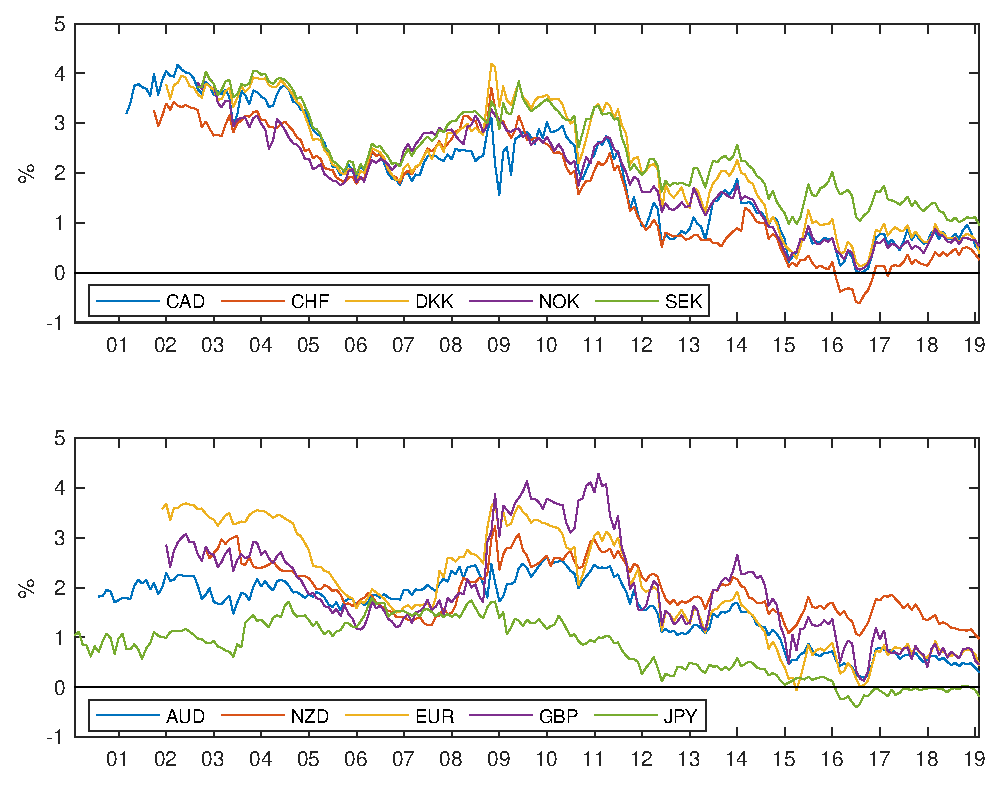
\includegraphics[width=1\textwidth,height=0.45\textheight]{../Figures/Temp/temp_tp10yrAE}
			\par\end{centering}
		\caption{Estimated 10-Year Term Premia: Advanced Economies.}\label{fig:temp_tp10yrAE}
	\end{figure}

According to KW, the 10-year term premium estimate for the U.S. has been negative for most of the time since mid-2011, fluctuating between $-1$\% and $0$. Of the advanced countries considered, only Switzerland and Japan have experienced more than one month with a negative term premium, compared to several emerging markets, mainly Korea, Russia and Turkey. In particular, before the taper tantrum there was a tendency of declining the term premia, which for some countries actually turned out negative.

\subsubsection{Term Structure of Term Premia}
In addition to comparing the term premia across countries, one can also compare them across maturities per country. In general, the term premium increases with maturity. As one would expect, when long-term bonds are seen as risky, investors require a higher compensation for holding them. This pattern, however, is not universal. Figure \ref{fig:temp_ts_tp} in the Appendix shows two examples. The exceptions for the general pattern are observed in both advanced and emerging countries. Even the KW estimates show that after the Great Recession the 1-year term premium has been above the 5- and 10-year term premia at some points.
%\footnote{Sometimes, the standard deviation of the term premia increases with maturity.}
%		\begin{figure}[!htbp]
		\begin{centering}
			\vspace{12.5mm}
			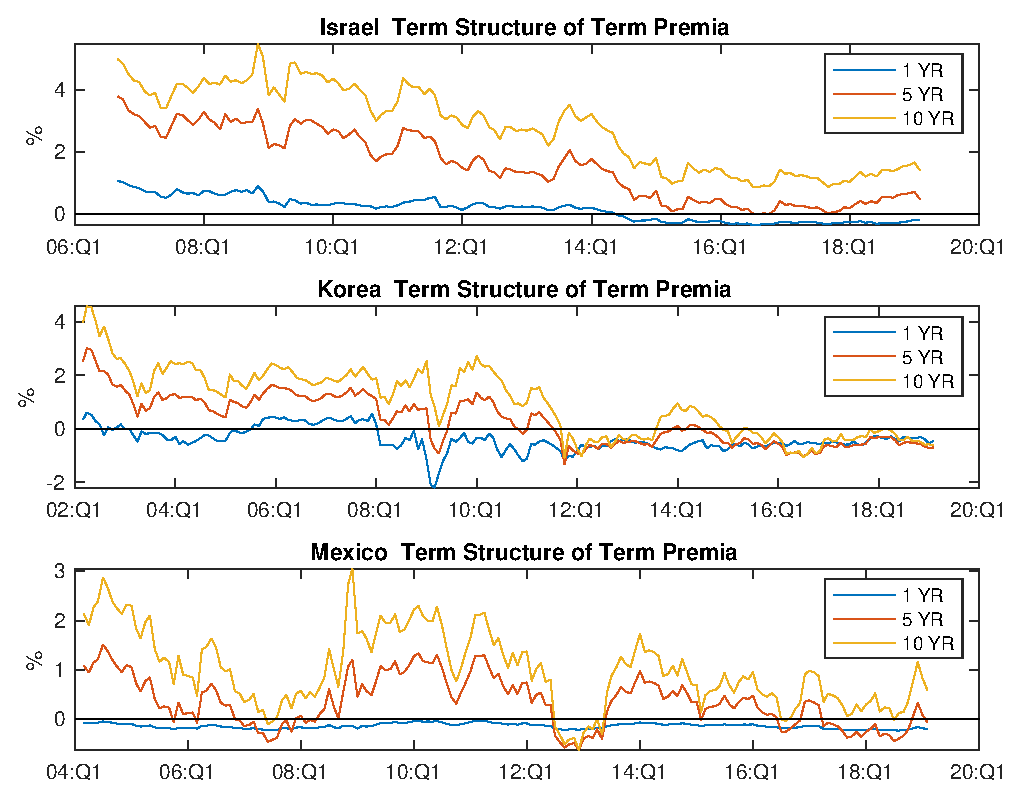
\includegraphics[width=1\textwidth,height=0.8\textheight]{../Figures/Temp/temp_ts_tp}
			\par\end{centering}
		\caption{Estimated Term Premia for Different Maturities.}\label{fig:temp_ts_tp}
	\end{figure}

\subsubsection{Common Factors in Term Premia}
To see whether there are common factors influencing the term premia in emerging markets, Table \ref{tab:temp_tp_common} shows the proportion of the total variation in the 10-year term premia explained by the first three PCs, with two different starting dates. To consider all countries, the first starting date is December 2006 and, to see if the results hold over a longer time period, the second starting date\footnote{For emerging markets, the second case only includes Colombia, Indonesia, Israel, Korea, Mexico, Philippines, South Africa and Turkey.} is June 2005. In both cases, the first three PCs explain more than $80\%$ of the variation in the term premia in emerging markets and more than $97\%$ for advanced countries. This evidence highlights the importance of considering global factors as drivers of the term premia. But at the same time, the evidence for emerging markets shows that both domestic and common factors seem to be at play as drivers of their term premia.
%	\begin{table}
	\centering
\begin{tabular}{l|cccc}
\toprule
&\textbf{PC1}&\textbf{PC2}&\textbf{PC3}&\textbf{Sum}\\\midrule
{ Since Nov 2016} - All Countries&40.29&23.62&12.37&76.28\\\
Since Jun 2005 - 8 countries&52.46&16.66&12.08&81.19\\ \bottomrule
\end{tabular}
\\
\caption{Proportion of Total Variance in 5yr RP Explained by First 3 PCs.}
\label{tab:pc_common}
\end{table}

%	\begin{footnotesize}\begin{table}\centering\begin{tabular}{l|cccc}
\toprule
\multicolumn{1}{c}{} &\multicolumn{2}{c}{EM TP}&\multicolumn{2}{c}{Residual}\\
\cmidrule(l{1.1em}r{1.1em}){2-3} \cmidrule(l{1.1em}r{1.1em}){4-5}
\multicolumn{1}{c}{} & 5 YR & 10 YR & 5 YR & 10 YR \\
\midrule
(15) Dec-06 & 67.40 & 71.67 & 62.99 & 58.25 \\(8)  Jul-05 & 79.57 & 82.65 & 74.36 & 76.40 \\(4)  Latam & 95.43 & 94.96 & 94.01 & 92.47 \\(5)  Asia & 90.19 & 91.43 & 88.52 & 87.98 \\(4)  Europe & 97.38 & 95.25 & 97.15 & 93.38 \\\bottomrule\end{tabular}\caption{Percent of Total Variance Explained by First 3 PCs.}\label{table:CmnFctrs}\end{table}\end{footnotesize}
	\begin{tiny}\begin{table}\centering\begin{tabular}{l|cc}\toprule & Dec-2006 \\\midrule EM & 81.01 \\AE & 98.07 \\\bottomrule\end{tabular}\caption{Total Variation Explained by First 3 PCs (\%): 10-Year Term Premium.}\label{tab:temp_tp_common}\end{table}\end{tiny}

\subsubsection{Survey-Based Term Premia}
As already mentioned, one way to check the term premium estimates obtained from affine term structure models is to use survey data since long-term surveys of professional forecasters can be used to obtain a model-free estimate of the term premium. Using this approach, the term premium is calculated as the difference between the long-term interest rate and the survey-expectation of the future short-term interest rate over the same horizon. Since the long-term expectations of the policy rate for emerging markets are not provided by Consensus Economics, they are approximated as explained in section \ref{sec:SurveyData}. Figure \ref{fig:temp_tp10yrSvy} displays the long-term term premium estimated in this way for most of the emerging markets considered in figure \ref{fig:temp_tp10yrEM}.
		\begin{figure}[!htbp]
		\begin{centering}
			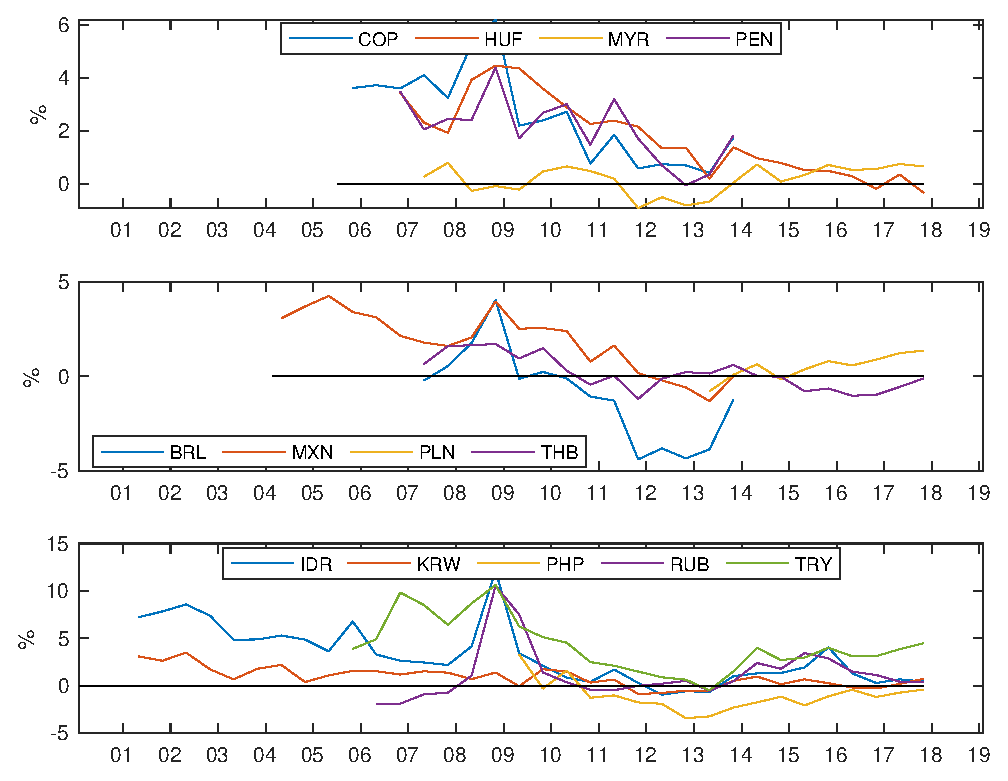
\includegraphics[width=1\textwidth,height=0.5\textheight]{../Figures/Temp/temp_tp10yrSvy}
			\par\end{centering}
		\caption{Survey-Based 10-Year Term Premium Estimates}\label{fig:temp_tp10yrSvy}
	\end{figure}

With the exception of Brazil during 2012-13, the term premia estimated using survey data is in line with the model-based term premia. In fact, the average correlation between the two is $80.4\%$.\footnote{Even for the term premia calculated using the nominal yield curve, the correlation with the survey-based term premia is equal to $85\%$.} This is reassuring and supports the idea of supplementing the term structure model with survey data to better pin down the term premia in emerging markets and provide a more robust decomposition of the nominal yield curve.


\section{Cyclical Properties of the Term Premia} \label{sec:correl}
\iftoggle{commentboxes}{% Defined in packages.tex
\gototoc
\begin{tabular}{|p{\linewidth}|}
	\hline
	\begin{itemize}
		\item Constrast the reference to Anaya et al. 2017 with Gilchrist, Yue \& Zakrajzek (2018) and with Wright et al. (2017).
		\item Contrast effect of FX with Hofman, Shim and Shin
		\item Claims about effect of variables on expected part can be tested using the expected part directly as well as forecasts.
	\end{itemize}
	\\ \hline
\end{tabular} \\}

Since this is the first time that term premia is estimated using synthetic yield curves, I first present their correlation with variables commonly associated with risk and uncertainty before proceeding to a more formal analysis.

%\subsection{Correlation with Financial Variables}
%Table \ref{tab:rp_reg_lvix} reports the regression of the term premia on $\ln \left( VIX \right)$. As it can be seen, the VIX plays a relevant role as the effect is significant for most of the countries. With the exception of Hungary and Malaysia, an increase in the VIX is associated with an increase in the term premia in emerging markets: a $10\%$ increase in the VIX increases the term premia by $10$ basis points on average. Based on the $R^2$, it explains more than $10\%$ of the variation in term premia for the countries for which the effect is higher.
%
%The effect of the federal funds rate is shown in Table \ref{tab:rp_reg_ffr}. It is significant in half of the countries. With the exception of Russia, an increase in the fed funds rate decreases the term premia by 25 basis points on average. It also explains more than $10\%$ of the variation in term premia for those countries. This is consistent with a flattening of the synthetic yield curve. Along with evidence that the monetary policy stance in emerging markets tend to move in the same direction than that in the U.S. \citep*{AnayaHachulaOffermanns:2017}, this is consistent with an increase in the expectation of future short-term interest rates in emerging markets.
%
%The exchange rate has an effect on the term premia of only four countries: Indonesia, Peru, Philippines and Russia. The results are reported in Table \ref{tab:rp_reg_rfx}. A $1\%$ depreciation of the LC is associated with a decrease in the term premia of 15 basis points on average for those countries. Along with the uncovered interest parity (according to which a LC depreciation would be followed by an increase in the short-term interest rate), this effect is also consistent with an increase in the expectation of future short-term interest rates.
%
%Unlike the previous financial variables, the return of the local stock market is not correlated with the term premia as shown in Table \ref{tab:rp_reg_stx}.\footnote{Since the countries studied are emerging markets, the return on the price of a commodity was also used as a regressor (in this case oil) but there was also no observed effect (not reported here).}

\subsection{Relationship with Risk and Uncertainty Measures}
To see how the term premia co-moves with variables associated with risk and uncertainty, they are compared against the 10-year U.S. term premium from KW, the LC credit spread from \cite{DuSchreger:2016a} or the convenience yield from \cite{DuImSchreger:2018}, and the economic policy uncertainty (EPU) index proposed by \citet*{BakerBloomDavis:2016}. The first variable is an indicator of global financial conditions, while the second is an indicator of credit risk for emerging markets or the convenience yield for advanced economies. The EPU index is based on the frequency of articles in local newspapers containing key words such as `economy', `uncertainty' and `central bank'; however, it is only available for 5 of the emerging markets in the sample. Tables \ref{tab:temp_tp_corr10yr} and \ref{tab:temp_tp_corr10yr_epu} show these correlations.
%	\begin{tiny}\begin{table}\centering\begin{tabular}{l|ccc}\toprule & US TP & LCCS & EPU \\\midrule BRL & 0.38 & - & -0.29 \\COP & 0.67 & 0.09 & 0.13 \\HUF & 0.01 & -0.27 & - \\IDR & 0.36 & -0.21 & - \\ILS & 0.75 & -0.16 & - \\MXN & 0.72 & 0.20 & -0.05 \\PEN & 0.63 & -0.34 & - \\PHP & 0.49 & -0.22 & - \\PLN & 0.58 & -0.12 & - \\TRY & 0.76 & -0.16 & - \\KRW & 0.59 & 0.02 & -0.07 \\MYR & 0.23 & -0.53 & - \\RUB & 0.46 & -0.46 & -0.47 \\THB & 0.57 & -0.76 & - \\ZAR & 0.21 & 0.15 & - \\\bottomrule\end{tabular}\caption{Correlations of 10-Year Term Premia.}\label{table:Correls10yr}\end{table}\end{tiny}
	\begin{tiny}\begin{table}
		\centering
		\begin{tabular}{l|ccc}
			\toprule
			 & TP-USTP & TP-CIP Dev
			\\\midrule 
			EM & 0.60 & -0.28 \\
			A-SOE & 0.80 & -0.01 \\
			G-3 & 0.71 & -0.29 \\
			\bottomrule
		\end{tabular}
		\caption{Correlations of 10-Year Term Premia: U.S TP and CIP deviations}\label{tab:temp_tp_corr10yr}\end{table}\end{tiny}
	\begin{tiny}\begin{table}
		\centering
		\begin{tabular}{l|ccccc}
			\toprule
			 & BRL & COP & KRW & MXN & RUB \\
			 \midrule 
			 TP-EPU & 0.14 & 0.46 & -0.32 & 0.40 & -0.22 \\
%			 $\perp$TP-EPU & 0.11 & 0.28 & -0.31 & 0.20 & -0.09 \\
			 \bottomrule
		 \end{tabular}
	 \caption{Correlations of 10-Year Term Premia: Economic Policy Uncertainty Index}\label{tab:temp_tp_corr10yr_epu}\end{table}\end{tiny}

The term premia in emerging markets is related to the U.S. term premium but not as tightly linked as those for advanced countries. To assess the relationship of the country-specific component of the term premia with the other two variables, I regress the term premium of each country on the U.S. term premium and use the residuals as the `idiosyncratic' term premium (i.e. the part of a country's term premium orthogonal to the U.S. term premium).

The correlation of the term premia with the deviations from CIP is negative. \cite{DuSchreger:2016a} show that the LC credit spread has a low reaction to global variables. This provides a possible explanation for the negative relationship between the term premia and the LC credit spread, since the former seems to react to global factors. The last column of table \ref{tab:temp_tp_corr10yr}  shows that once the term premia in emerging markets is purged from the effect of the U.S. term premium, the relationship is still negative but the magnitude declines. The opposite is observed for advanced small open economies but remember that for them the deviations from CIP reflect a convenience yield.

The term premia for Latin American countries show a positive correlation with the EPU index; the correlation for Korea and Russia, however, is negative. The relationship might be related to the fact that after the Great Recession, the term premia for both countries has been negative during a considerable period as shown in figure \ref{fig:temp_tp10yrEM}. This can be verified if the EPU index for countries with a similar situation like Turkey becomes available. The sign of the relationship with the idiosyncratic component of the term premia holds but the magnitude declines.

%\subsection{Correlation with Macroeconomic Variables}
%Three variables that are closely followed by market participants are inflation, the unemployment rate and industrial production because they capture the state of the economy at a monthly frequency. Therefore, the macroeconomic variables used in this section are the year-on-year percentage change in the consumer price index, the unemployment rate and the year-on-year percentage change in industrial production in each country. All countries have at least two of the three variables available for their respective time span, and only seven countries have the three variables available during their whole sample period.\footnote{The seven countries are Colombia, Hungary, Korea, Mexico, Peru, Russia and Turkey. Inflation is not included for Philippines since it is available starting in January 2013. Unemployment is not included for Israel (available since January 2012), Poland (March 2010) and South Africa (March 2008). Industrial production is not included for Indonesia (January 2011), Malaysia (January 2013) and Thailand (February 2011).} 
%
%The available macroeconomic variables are included in the regressions at the same time. The results are reported in Table \ref{tab:rp_reg_macro}. The table shows that inflation and the unemployment rate are important drivers of the term premia. They are significant for all countries for which they are included. An increase in inflation tends to decrease the term premia by 12 basis points on average, while unemployment increases term premia by 50 basis points on average. These effects are consistent with an active monetary policy in line with the standard textbook mechanism and expectations of future short-term interest rates following the same direction of the policy rate. Industrial production is important statistically and economically only for Peru.
%
%In addition, the variation in term premia explained by these variables is relatively high, $34\%$ on average, which is higher than for any of the financial variables analyzed before. This supports including macroeconomic factors in the vector of state variables. In future versions, this can be done following \citet*{JPS:2014}, which will also help in further testing the relevance of unspanned or hidden factors in emerging markets.

\subsection{Drivers of Term Premia}
To study the cyclical properties of term premia in emerging markets formally, I run  panel data regressions with a variety of macroeconomic and financial variables. The macroeconomic variables considered have a monthly frequency, and since the financial variables considered are available daily, end-of-month values are used for them.

The panel data regressions have the form

\begin{equation} \label{eq:panel_reg}
	tp_{it} = \alpha_{i} + \beta' z_{it} + u_{it},
\end{equation}

where $tp_{it}$ denotes the model-based 10-year term premium of country $i$ in month $t$, $z_{it}$ is a vector of regressors and $\alpha_{i}$ denotes a country fixed-effect. The regressors include global and domestic variables as suggested by the evidence presented in table \ref{tab:temp_tp_common}.

The global financial variables include the Cboe VIX, the federal funds rate, the S\&P $500$ index and the oil price. The VIX and the federal funds rate have been used in the global financial cycle literature \citep[see][]{Rey:2013} to study the effects of common factors on capital flows. The VIX is usually used as a measure of risk aversion and economic uncertainty and the fed funds rate is a measure of the monetary policy stance in the U.S. Given the sudden spikes in the VIX, it is common to use the $\ln \left( VIX \right)$ instead of the VIX directly. For the U.S. monetary policy, the variable used is the effective federal funds rate calculated by the New York Fed. 
 
 The domestic variables include inflation, the unemployment rate and industrial production to capture macroeconomic effects. In addition, the exchange rate (LC per USD) and the local stock market index are used as measures of local financial conditions. For this two variables, both levels and monthly returns are used.\footnote{The monthly returns are calculated as the log difference of the series.} Given the different scales, the exchange rate is standardized when used in levels.

Table \ref{tab:temp_tp_regs} reports different specifications of the model in equation (\ref{eq:panel_reg}). The first model in the table focuses mainly on global variables, while the second one focuses on domestic variables. These two models already shed some light on the driving forces behind the term premia in emerging markets. However, the models with the most explanatory power include both global and domestic variables.
%	\begin{tiny}\begin{tabular}{cccccc}
\toprule
log(VIX)& 0.021&-0.195&& 0.538***& 0.513***\\\
 &(0.33)&(0.32)&&(0.15)&(0.14)\\\
FFR&-0.198***& 0.009&&-0.149*& 0.109\\\
 &(0.08)&(0.08)&&(0.08)&(0.09)\\\
USTP10&& 0.546***&&& 0.639***\\\
 &&(0.06)&&&(0.06)\\\
SPX&-0.001***&-0.000&&-0.001***&\\\
 &(0.00)&(0.00)&&(0.00)&\\\
INF&&&-0.090&-0.136**&-0.150**\\\
 &&&(0.07)&(0.06)&(0.05)\\\
UNE&&& 0.160& 0.047& 0.029\\\
 &&&(0.12)&(0.10)&(0.09)\\\
IP&&&-0.008& 0.002&-0.001\\\
 &&&(0.01)&(0.01)&(0.01)\\\
Country FE&Yes&Yes&Yes&Yes&Yes\\\
Observations&2483&2483&1757&1757&1757\\\
Countries&15&15&15&15&15\\\
Within $R^2$&0.15&0.23&0.07&0.26&0.38\\\
\end{tabular}
\end{tiny}
	% Preview source code for paragraph 0
\begin{scriptsize}
% Preview source code for paragraph 0
\begin{table}
\begin{center}
\begin{tabular}{lr@{\extracolsep{0pt}.}lr@{\extracolsep{0pt}.}lr@{\extracolsep{0pt}.}lr@{\extracolsep{0pt}.}lr@{\extracolsep{0pt}.}lr@{\extracolsep{0pt}.}l}
	\hline 
 & \multicolumn{2}{c}{(1)} & \multicolumn{2}{c}{(2)} & \multicolumn{2}{c}{(3)} & \multicolumn{2}{c}{(4)} & \multicolumn{2}{c}{(5)} & \multicolumn{2}{c}{(6)}\tabularnewline
	\hline 
	& \multicolumn{2}{c}{} & \multicolumn{2}{c}{} & \multicolumn{2}{c}{} & \multicolumn{2}{c}{} & \multicolumn{2}{c}{} & \multicolumn{2}{c}{}\tabularnewline
	log(VIX) & 0&20 & \multicolumn{2}{c}{} & 0&26 & 0&24 & 0&65{*}{*}{*} & 0&10\tabularnewline
	& (0&35) & \multicolumn{2}{c}{} & (0&24) & (0&16) & (0&21) & (0&19)\tabularnewline
	FFR & 0&07 & \multicolumn{2}{c}{} & 0&23{*}{*} & 0&13 & 0&22{*}{*} & 0&11\tabularnewline
	& (0&11) & \multicolumn{2}{c}{} & (0&09) & (0&09) & (0&10) & (0&10)\tabularnewline
	USTP10 & 1&49{*}{*}{*} & \multicolumn{2}{c}{} & \multicolumn{2}{c}{} & 1&30{*}{*}{*} & \multicolumn{2}{c}{} & 1&22{*}{*}{*}\tabularnewline
	& (0&20) & \multicolumn{2}{c}{} & \multicolumn{2}{c}{} & (0&12) & \multicolumn{2}{c}{} & (0&16)\tabularnewline
	S\&P & -0&00 & \multicolumn{2}{c}{} & -0&00{*} & \multicolumn{2}{c}{} & \multicolumn{2}{c}{} & \multicolumn{2}{c}{}\tabularnewline
	& (0&00) & \multicolumn{2}{c}{} & (0&00) & \multicolumn{2}{c}{} & \multicolumn{2}{c}{} & \multicolumn{2}{c}{}\tabularnewline
	Oil & -0&01{*} & \multicolumn{2}{c}{} & 0&00 & \multicolumn{2}{c}{} & \multicolumn{2}{c}{} & \multicolumn{2}{c}{}\tabularnewline
	& (0&01) & \multicolumn{2}{c}{} & (0&00) & \multicolumn{2}{c}{} & \multicolumn{2}{c}{} & \multicolumn{2}{c}{}\tabularnewline
	Inflation & \multicolumn{2}{c}{} & 0&26{*}{*}{*} & 0&19{*}{*}{*} & 0&19{*}{*}{*} & 0&22{*}{*}{*} & 0&21{*}{*}{*}\tabularnewline
	& \multicolumn{2}{c}{} & (0&05) & (0&06) & (0&05) & (0&05) & (0&05)\tabularnewline
	Unemployment & \multicolumn{2}{c}{} & 0&21{*}{*}{*} & 0&17{*}{*} & 0&13{*}{*} & 0&21{*}{*}{*} & 0&13{*}{*}\tabularnewline
	& \multicolumn{2}{c}{} & (0&07) & (0&06) & (0&05) & (0&06) & (0&05)\tabularnewline
	IP & \multicolumn{2}{c}{} & -0&01 & -0&01 & -0&02 & -0&02 & -0&02{*}\tabularnewline
	& \multicolumn{2}{c}{} & (0&01) & (0&01) & (0&01) & (0&01) & (0&01)\tabularnewline
	zFX & \multicolumn{2}{c}{} & 0&21{*} & 0&41{*}{*} & 0&29{*}{*} & \multicolumn{2}{c}{} & \multicolumn{2}{c}{}\tabularnewline
	& \multicolumn{2}{c}{} & (0&11) & (0&15) & (0&10) & \multicolumn{2}{c}{} & \multicolumn{2}{c}{}\tabularnewline
	Stock Market & \multicolumn{2}{c}{} & -0&00{*}{*} & -0&00 & -0&00 & \multicolumn{2}{c}{} & \multicolumn{2}{c}{}\tabularnewline
	& \multicolumn{2}{c}{} & (0&00) & (0&00) & (0&00) & \multicolumn{2}{c}{} & \multicolumn{2}{c}{}\tabularnewline
	Return S\&P & \multicolumn{2}{c}{} & \multicolumn{2}{c}{} & \multicolumn{2}{c}{} & \multicolumn{2}{c}{} & 0&00 & -0&01\tabularnewline
	& \multicolumn{2}{c}{} & \multicolumn{2}{c}{} & \multicolumn{2}{c}{} & \multicolumn{2}{c}{} & (0&01) & (0&01)\tabularnewline
	Return Oil & \multicolumn{2}{c}{} & \multicolumn{2}{c}{} & \multicolumn{2}{c}{} & \multicolumn{2}{c}{} & 0&00 & 0&00\tabularnewline
	& \multicolumn{2}{c}{} & \multicolumn{2}{c}{} & \multicolumn{2}{c}{} & \multicolumn{2}{c}{} & (0&00) & (0&00)\tabularnewline
	Return FX & \multicolumn{2}{c}{} & \multicolumn{2}{c}{} & \multicolumn{2}{c}{} & \multicolumn{2}{c}{} & 0&02{*} & 0&01\tabularnewline
	& \multicolumn{2}{c}{} & \multicolumn{2}{c}{} & \multicolumn{2}{c}{} & \multicolumn{2}{c}{} & (0&01) & (0&01)\tabularnewline
	Return Stocks & \multicolumn{2}{c}{} & \multicolumn{2}{c}{} & \multicolumn{2}{c}{} & \multicolumn{2}{c}{} & 0&00 & 0&00\tabularnewline
	& \multicolumn{2}{c}{} & \multicolumn{2}{c}{} & \multicolumn{2}{c}{} & \multicolumn{2}{c}{} & (0&01) & (0&01)\tabularnewline
	Constant & 2&01 & -0&65 & -0&44 & -1&03 & -3&18{*}{*}{*} & -0&73\tabularnewline
	& (1&66) & (0&63) & (1&41) & (0&85) & (0&93) & (0&80)\tabularnewline
	& \multicolumn{2}{c}{} & \multicolumn{2}{c}{} & \multicolumn{2}{c}{} & \multicolumn{2}{c}{} & \multicolumn{2}{c}{} & \multicolumn{2}{c}{}\tabularnewline
	Observations & \multicolumn{2}{c}{2,407} & \multicolumn{2}{c}{1,969} & \multicolumn{2}{c}{1,969} & \multicolumn{2}{c}{1,969} & \multicolumn{2}{c}{1,969} & \multicolumn{2}{c}{1,969}\tabularnewline
	R-squared & 0&32 & 0&32 & 0&39 & 0&53 & 0&34 & 0&49\tabularnewline
	Number of Countries & \multicolumn{2}{c}{15} & \multicolumn{2}{c}{15} & \multicolumn{2}{c}{15} & \multicolumn{2}{c}{15} & \multicolumn{2}{c}{15} & \multicolumn{2}{c}{15}\tabularnewline
	Country FE & \multicolumn{2}{c}{Yes} & \multicolumn{2}{c}{Yes} & \multicolumn{2}{c}{Yes} & \multicolumn{2}{c}{Yes} & \multicolumn{2}{c}{Yes} & \multicolumn{2}{c}{Yes}\tabularnewline
	\hline 
	\multicolumn{13}{l}{Robust standard errors in parentheses; {*}{*}{*} p$<$0.01, {*}{*} p$<$0.05,
		{*} p$<$0.1.}\tabularnewline
\end{tabular}\caption{Panel Data Regressions of the 10-Year Term Premium (\%).} \label{tab:temp_tp_regs}
\end{center}
\end{table}
\end{scriptsize}


The main global factor is the U.S. term premium, and the two main domestic factors are inflation and unemployment. Holding the other factors constant, an increase in any of these three variables increases the term premia in emerging markets but the greatest influence comes from the external variable not from domestic ones; that is, external conditions have a relevant impact on domestic bond markets. This is in line with the literature studying the global financial cycle that focuses on capital flows. However, the channel does not seem to be through the VIX nor even through the monetary policy of the U.S. directly via the federal funds rate but through the U.S. term premia. Both the VIX and the federal funds rate have a positive effect on the term premia in emerging markets but the effect disappears once the U.S. term premium is included in the regressions. An increase in the U.S. term premium translates into a more than proportional increase in the term premium of emerging markets.

The effect of the domestic variables is in line with what has been found for advanced countries using nominal yield curves. Investors demand a higher term premium during recessions, when the unemployment rate increases. This provides evidence of a countercyclical behavior of the term premia in emerging markets. Moreover, the positive effect of inflation on the term premia conforms with the idea that inflation erodes the value of nominal bonds and so in periods of rising inflation investors demand a higher term premium. The effect of both variables is broadly similar across models. 

Finally, the exchange rate also seems to be playing a role; a depreciation of the local currency is associated with an increase in the term premium. This seems counterintuitive since emerging markets are usually commodity exporters so it appears to contradict the standard trade-channel effect. However, it is in line with the risk-taking channel of exchange rates found by \cite{HofmannShimShin:2017}, according to which currency appreciation is associated with easier financial conditions and compressed sovereign bond spreads.

\section{Conclusions}\label{sec:conclusions}
\iftoggle{commentboxes}{% Defined in packages.tex
\gototoc
\begin{tabular}{|p{\linewidth}|}
	\hline
	\begin{itemize}
		\item Study how the effect of macroeconomic and financial variables on the term premia compare to their effect on the LC credit spread and on the expectation of future short-term interest rates. That is, perform a full decomposition of `observed' yields (default risk, term premia and expectations of future short-term interest rates) and analyze the effects of said variables on each component. This would extend the analysis done by GilchristYueZakrajsek:2018 on the spillover effects of U.S. monetary policy on LC bonds of emerging markets. Compare also with HofmannShimShin:2017. The set of variables could be extended too (e.g. monetary policy shocks in other advanced economies).
		
		\item Perform a more robust analysis of the determinants of term premia in emerging markets and how they differ from those of advanced economies.
		
		\item Uncovered interest parity is based on risk-neutrality. Could the risk-neutral yields obtained from the term structure model be used to revisit the findings from the literature on deviations from uncovered interest parity for EMs? This will extend the work done by AngChen:2010.
		
		\item Can the findings from this research be used to make a decomposition of the FC-denominated yield curve? Following the same strategy of using synthetic yield curves. Similar to the way it can be done for the U.S. yield curve, the FC yield curve can be swapped into LC, which would allow a comparison between the FC and the LC yield curves. Can this be related to exchange rates and inflation expectations? To sovereign risks?
		
		\item The estimated yield curves are an input to the decomposition of the changes in the exchange rates (risk premia, inflation expectations) done by StavrakevaTang:2018b for advanced economies, which could be extended for emerging markets.
		
		\item Exploit the cross-section of yields by using a multi-country term structure model in order to improve the precision in the term premia estimates. In future versions, a multi-country affine term structure model may be used in the spirit of JotikasthiraLeLundblad:2015 to exploit information in the cross-section of yield curves.
		
		\item Forecast the LC yields in emerging markets.
	\end{itemize}
	\\ \hline
\end{tabular} \\}

This paper estimates the term premia for 15 emerging markets using synthetic yield curves. The LC credits spread accounts for the difference between the nominal and the synthetic yield curve. By accounting for credit risk, this paper avoids violating the risk-free assumption underlying affine term structure models.

Exploiting the flexibility of these models, I decompose the synthetic yield curve into an expectation for the future short-term interest rate and a term premium, which in turn allows to decompose the nominal yield curve into three components (the third one being the LC credit spread).

The evidence presented in this paper shows that the term premia in emerging markets is around 175 basis points on average, higher than the average of the LC credit spread of 85 basis points. The results are compared to those obtained from surveys of professional forecasters and from advanced countries to establish a set of stylized facts. It is shown that the benefits of using synthetic yield curves are greater for emerging markets than for advanced economies, which implies that the terms `risk premium' and `term premium' should not be used interchangeably, at least for emerging markets. The analysis also shows that the phenomenon of a negative term premium has been observed more often for some emerging markets than for advanced countries.

The analysis shows that not only common factors influence the term premia in emerging markets but also domestic ones. In particular, the U.S. term premium is the main driver, having a more than proportional effect on their term premia. The evidence also shows a countercyclical behavior of the term premia with domestic business cycles and a positive relationship with inflation, in line with the idea that it erodes the value of nominal bonds.

The work presented in this paper can be extended in several directions and I will continue working on them. First, as already indicated, the information from survey data can aid in mitigating the identification problem in affine term structure models, which translates into more robust estimates of the term premia. As a consequence, the decomposition of the nominal yield curve will also be more robust so that it can provide useful information for the analysis of monetary policy in emerging markets.

Different models can also be used to assess different characteristics of the data from the synthetic curves. A model that explicitly considers the joint behavior of nominal and real interest rates can allow to further decompose both nominal and synthetic yield curves into the expectation of the future real interest rate and the real term premium. The model can also be supplemented not only with survey data but also with macroeconomic information. Other extensions include models with jumps in yields, which might be applicable to a couple of emerging markets (those with a poor fit mentioned in section \ref{sec:results}). Given the reaction to common factors, multi-country term structure models might be relevant. To further study the phenomenon of negative term premiums, quadratic term structure models with joint dynamics for stocks and bonds might be useful.

Finally, minor improvements can also be included like extending the comparison with advanced economies for the analysis shown in section \ref{sec:correl}. In particular, analyzing the relationship between the EPU index for those advanced countries for which it is available (Australia, Canada, Germany, Japan, UK and Sweden) to compare it with what is reported for emerging markets, as well as contrasting the results from the panel regressions to advanced countries. More generally, the panel regression analysis can be applied to the other components of the nominal yield curve, namely the expectation part and the LC credit spread. This will provide a broader picture of the effects of global factors on local bond markets.
